\subsection{Struttura del sito}
Ogni pagina del sito è formata dai seguenti elementi:
\begin{itemize}
	\item Header;
	\item breadcrumb;
	\item box che permette il login o mostra l'account con cui si è autenticati;
	\item menù;
	\item contenuto della pagina;
	\item footer.
\end{itemize}

\subsubsection{Mappa del sito}
\begin{figure}[H]
	\centering
	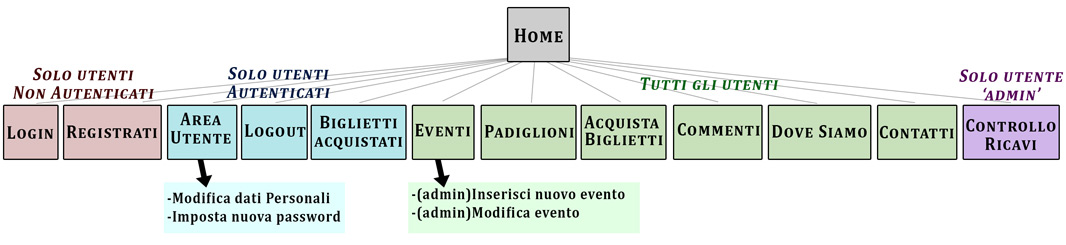
\includegraphics[width=16cm]{mappa-sito-small}
	\caption{Mappa del sito.}
\end{figure}
Oltre alla home page, che è concettualmente la radice del sito ed è ovviamente accessibile a tutti gli utenti, le varie pagine sono concettualmente suddivise nelle seguenti aree basate sull'attore che le andrà ad utilizzare:
\begin{itemize}
	\item Per soli utenti non autenticati;
	\item per soli utenti autenticati;
	\item per tutti gli utenti;
	\item per il solo utente amministratore.
\end{itemize}

\paragraph{Home page}
È, concettualmente, la radice del sito, nonché la pagina in cui l'utente si dovrebbe ritrovare quando si collega al sito. Contiene un paragrafo introduttivo di benvenuto e presentazione, seguito dalle news riguardante l'evento.

\paragraph{Per soli utenti non autenticati}
Quest'area contiene le pagine destinate agli utenti non autenticati, permettendo loro di interagire con le funzioni di autenticazione e registrazione al sito.
Pagine che ne fanno parte:
\begin{itemize}
	\item Login;
	\item Registrazione.
\end{itemize}

\paragraph{Per soli utenti autenticati}
Quest'area contiene le pagine che possono essere visitate o accedute solo dagli utenti che hanno eseguito l'autenticazione al sito. Le pagine di questa area permettono di interagire con gli aspetti relativi alla gestione del proprio account, come ad esempio la modifica dei dati personali o della password, la possibilità di effettuare il logout e, infine, un elenco dei biglietti acquistati da quell'account. L'accesso ad una di queste pagine da parte di un utente non autenticato produce un errore oppure, nel caso di area utente e logout, un reindirizzamento. Inoltre, ad un utente non autenticato non sono mai mostrati collegamenti a queste pagine.
Pagine che ne fanno parte:
\begin{itemize}
	\item Area Utente;
	\item Logout;
	\item Biglietti Acquistati.
\end{itemize}

\paragraph{Per tutti gli utenti}
Queste pagine sono accessibili a tutti gli utenti, a prescindere dal loro stato di autenticazione, tramite il menù.
Contengono i contenuti veri e propri del sito, con informazioni sulla fiera, l'acquisto dei biglietti e la possibilità di lasciare dei commenti.
Pagine che ne fanno parte:
\begin{itemize}
	\item Eventi:
		Presenta la lista di tutti gli eventi che si terranno nel corso della fiera. Per ogni evento vengono offerte informazioni utili quali la data, l'ora di inizio, l'ora di fine, il padiglione in cui si svolgeranno ed una descrizione.
		L'utente amministratore ha la possibilità di svolgere alcune funzioni aggiuntive: l'inserimento di un nuovo evento e la modifica o cancellazione di un evento già inserito.
	\item Padiglioni:
		Mostra l'elenco dei padiglioni presenti nella fiera suddivisi per settori. Inoltre mostra anche una mappa con la posizione di ogni padiglione. Il contenuto è uguale per tutte le categorie di utenti.
	\item Acquista biglietti:
		Elenca a tutti i tipi di utenti le varie tipologie di biglietti disponibili ed il loro prezzo. Ad un utente autenticato offre anche la possibilità di procedere all'acquisto di uno o più biglietti.
	\item Commenti:
		Rappresenta il "libro ospiti" del sito. Gli utenti di tutte le categorie possono leggere i commenti. Un utente autenticato ha a disposizione la funzione di eliminazione per i commenti da lui inviati, mentre l'utente amministratore può eliminare qualsiasi commento.
	\item Dove siamo:
		Offre indicazioni per raggiungere il luogo della fiera. Il contenuto è uguale per tutte le categorie di utenti.
	\item Contatti:
		Contiene informazioni su come contattare gli organizzatori della fiera. Il contenuto è uguale per tutte le categorie di utenti.
\end{itemize}

\paragraph{Per il solo utente amministratore}
A questa categoria appartiene una sola pagina: Controllo ricavi.
Questa pagina è destinata all'utente amministratore e presenta in forma tabellare il resoconto sui biglietti venduti e sui guadagni.

\subsection{Layout}
Per quanto riguarda il layout del sito, è stato scelto di adottare schema a tre pannelli (con breadcrumb), costituito da un header per l’intestazione del sito e la barra di navigazione, un footer, un menu di navigazione a sinistra: questo si riflette bene nell'organizzazione del nostro codice a template.
Sono state inoltre previste due tipologie principali di visualizzazione: una per i normali schermi di desktop/notebook ed una per i dispositivi mobile (o comunque con lo schermo di risoluzione ridotta). \newline
La versione mobile presenta un layout verticale, dove viene visualizzato prima l'header, poi il menu, quindi il body, ed infine il footer.

\subsection{Scelte progettuali}
Dato che la fascia d'utenza individuata risulta essere disomogenea in fatto di età e prevedendo utenti con più di 50 anni, è stato pensato di rendere il sito il più semplice ed intuitivo possibile. Di conseguenza, si è cercato di mantenere il design quanto più semplice e minimale possibile, e suddividere il sito in un numero relativamente limitato di pagine. Inoltre, ogni pagina ha un nome che la identifica in modo chiaro e ha dei contenuti specifici e strettamente correlati al titolo. Per agevolare la navigazione sono stati inseriti dei link dove necessario per completare operazioni evitando disorientamento, come ad esempio un link alla pagina di login di fianco al messaggio che informa l'utente della necessità di autenticarsi per usufruire di una funzione del sito. \newline
Infine, data la sempre crescente diffusione dei dispositivi mobile, è stata posta particolare attenzione nel rendere il sito fruibile anche utilizzando questi dispositivi. 
	